\documentclass[conference,a4paper]{APSIPA2026}
\usepackage{cite}
\usepackage{amsmath,amssymb,amsfonts}
\usepackage{graphicx}
\usepackage{textcomp}
\usepackage{xcolor}
\definecolor{figblue}{RGB}{37,84,160}
\definecolor{figred}{RGB}{198,58,45}
\usepackage{booktabs}
\usepackage{array}
\usepackage{multirow}
\usepackage{tikz}
\usetikzlibrary{shapes.geometric,arrows.meta,positioning,calc}
\usepackage{url}
\usepackage{geometry}
\geometry{a4paper, top=19mm, bottom=43mm, right=13mm, left=13mm}
\usepackage{fancyhdr}
\renewcommand{\headrulewidth}{0pt}
\renewcommand{\footrulewidth}{0pt}
\fancypagestyle{firststyle}{%
  \fancyhf{}%
  \fancyhead[C]{2026 Asia Pacific Signal and Information Processing Association Annual Summit and Conference (APSIPA ASC)}%
}
\usepackage[hidelinks]{hyperref}
\graphicspath{{figs/}}
% Float placement: keep every figure and table inside the section that declares
% it. The defaults reserve so much of each column for text that a dense paper
% defers floats across section boundaries.
\renewcommand{\topfraction}{0.92}
\renewcommand{\bottomfraction}{0.85}
\renewcommand{\textfraction}{0.06}
\renewcommand{\floatpagefraction}{0.72}
\setcounter{topnumber}{3}
\setcounter{bottomnumber}{2}
\setcounter{totalnumber}{5}
% Tighten the space reserved around floats: this paper is float-dense, and the
% class defaults reserve ~20pt above and below each one.
\setlength{\textfloatsep}{8pt plus 2pt minus 2pt}
\setlength{\floatsep}{8pt plus 2pt minus 2pt}
\setlength{\intextsep}{8pt plus 2pt minus 2pt}
\setlength{\dblfloatsep}{8pt plus 2pt minus 2pt}
\setlength{\dbltextfloatsep}{10pt plus 2pt minus 2pt}

\begin{document}

\title{An Area-Optimized 8-bit Deep Learning Accelerator\\for GAN Image Generation on GF180MCU}

\author{
\IEEEauthorblockN{William Anthony, I~Made~Medika~Surya~W.M., John~Ruben~Saragi, Mahardhika~Putra~Adipratama,\\
Fairuz~Aquilla~Rahagi, Trio~Adiono, and Infall~Syafalni}
\IEEEauthorblockA{Bandung Institute of Technology, Bandung, Indonesia \\
E-mail: \{13223048, 13222021, 13222049, 13222081, 13222107\}@mahasiswa.itb.ac.id, \\
tadiono@itb.ac.id, infall@ieee.org}
}

\maketitle
\thispagestyle{firststyle}
\pagestyle{empty}

\begin{abstract}
This paper presents an area-optimized 8-bit deep learning accelerator for a small GAN image generator, hardened through a fully open-source flow on the open GF180MCU 180~nm process. The network is a three-layer MNIST multi-layer-perceptron generator, quantized to signed 8-bit integers and mapped onto a structural $4\times4$ processing-element array of native accumulation depth $K=256$. Starting from an eleven-macro predecessor, the result buffer is folded from three $256\times8$ SRAM macros used as byte planes into a single $64\times8$ macro addressed along the plane axis, cutting that buffer 77\% and the macro count to nine on a $3\times3$ grid and a $1375\times1325~\mu$m die. The result is \textbf{24\% less die area and 18\% less power, with more setup margin}, for 11.7\% more compute cycles per image. Antenna closure needed a method the usual density sweep could not supply: the sweep plateaued at one residual net, but the violating net names identified a single SRAM macro whose column broadcast sat too far from the array, and swapping it with the small result buffer reached zero violations at two independent densities. The macro signs off with zero DRC, LVS, XOR, and antenna violations at 40~ns across nine STA corners, verified bit-exactly up to a full 784-pixel image through the routed netlist.
\end{abstract}

\begin{IEEEkeywords}
Deep learning accelerator, GF180MCU, SRAM macro, area optimization, antenna closure, INT8 quantization, GAN, ASIC, LibreLane, open-source EDA.
\end{IEEEkeywords}

\section{Introduction}
Generative Adversarial Networks are a compact workload for testing neural inference on custom hardware. The generator used here is a small MNIST multi-layer perceptron turning a 64-dimensional latent vector into a $28\times28$ image; its arithmetic is dense matrix multiplication, so it maps onto a small array of multiply--accumulate units. An earlier version expressed this as behavioral loops and register memory arrays --- convenient for checking the algorithm, but not implementable, since buffers inferred as standard-cell registers make the design too large to route. It was restructured into a structural accelerator with a processing-element (PE) array, SRAM-backed buffers, and a controller, and hardened with eleven $256\times8$ SRAM macros on a $1600\times1500~\mu$m die.

This paper questions that design's memory rather than accepting it. Three of its eleven macros held the result buffer as byte planes of one 24-bit word, storing 48 bytes in 768 --- 6.25\% occupancy, on a buffer the array geometry fixes at sixteen accumulators forever. Folding those planes onto the address axis of one $64\times8$ macro recovers 77\% of that area and lets the die shrink. The contributions are: (1)~a memory-folding transformation cutting die area 24\% and power 18\% while \emph{improving} setup margin, at a measured cost in cycles; (2)~an antenna-closure method for when a density sweep plateaus --- read the violating net names to find a mis-placed macro instead of re-rolling placement --- confirmed by two independent levers reaching zero; (3)~a measured latency breakdown from per-stage cycle counts to end-to-end time over the host link; and (4)~a measured justification of INT8 against INT4, INT16, and FP16.

\section{Related Work}
Most neural accelerators are arrays of multiply-and-accumulate units --- the systolic TPU \cite{tpu} at large scale, surveyed broadly in \cite{survey} --- and running a floating-point network on an integer array normally uses the per-tensor quantization scale of Jacob et al. \cite{jacob}. The fabricated reference points span three orders of magnitude: DianNao \cite{diannao}, Eyeriss \cite{eyeriss} with its row-stationary dataflow, and, closer to our scale, Wang et al. \cite{wang}, all closed-PDK designs on commercial nodes. The comparison that matters most is OpenSpike \cite{openspike}, a spiking accelerator in open SkyWater 130~nm with open EDA and OpenRAM memory: same open-flow premise, different workload and memory strategy (Table~\ref{tab:compare}). The workload is a pretrained MLP GAN \cite{goodfellow, ganpretrained}; the RTL builds on the open DLA Engine project \cite{dlaengine}.

\section{GAN Architecture}\label{sec:overview}

\begin{figure*}[!t]
\centering
\resizebox{\textwidth}{!}{%
\begin{tikzpicture}[x=1mm,y=1mm,
  outerblk/.style={draw=figblue,fill=figblue!4,rounded corners=2.5mm,line width=1pt},
  subblk/.style={draw=figblue!60,fill=white,rounded corners=1.6mm,line width=0.6pt},
  syn/.style={figblue!45,line width=0.3pt},
  flow/.style={-{Stealth[length=1.9mm,width=1.6mm]},figblue,line width=0.9pt},
  ax/.style={-{Stealth[length=1.2mm,width=1.1mm]},black!55,line width=0.4pt},
  fn/.style={figred,line width=1.1pt},
  ttl/.style={font=\scriptsize\bfseries,text=figblue!80!black},
  dim/.style={font=\tiny,text=black!60},
  cell/.style={draw=figblue!75!black,line width=0.35pt,minimum size=3.4mm,inner sep=0pt,font=\tiny}]
% ---- top-level blocks ----
\draw[outerblk] (0,-14) rectangle (19,14);
\draw[outerblk] (26,-15) rectangle (154,19);
\draw[outerblk] (161,-14) rectangle (181,14);
\node[font=\small\bfseries,text=figblue!80!black] at (90,16.1) {MLP GAN Generator};
% ---- fat arrows between top-level blocks ----
\draw[draw=figblue,fill=figblue!15,line width=0.8pt]
  (19.9,1.0) -- (23.2,1.0) -- (23.2,2.1) -- (25.3,0) -- (23.2,-2.1) -- (23.2,-1.0) -- (19.9,-1.0) -- cycle;
\draw[draw=figblue,fill=figblue!15,line width=0.8pt]
  (154.7,1.0) -- (158.0,1.0) -- (158.0,2.1) -- (160.1,0) -- (158.0,-2.1) -- (158.0,-1.0) -- (154.7,-1.0) -- cycle;
\node[dim] at (157.4,3.9) {reshape};
% ---- latent vector, drawn as a vector ----
\node[ttl,align=center] at (9.5,10.6) {Latent\\Vector};
\foreach [count=\i] \val/\sh in {0.8/45, -0.3/14, 1.2/60, -0.7/38}
  \node[cell,fill=figblue!\sh] at (9.5,{4.6-(\i-1)*3.4}) {$\val$};
\node[font=\tiny] at (9.5,-8.15) {$\vdots$};
\node[cell,fill=figblue!28] at (9.5,-10.6) {$0.5$};
\draw[line width=0.5pt,black!75] (7.2,6.6) -- (6.5,6.6) -- (6.5,-12.6) -- (7.2,-12.6);
\draw[line width=0.5pt,black!75] (11.8,6.6) -- (12.5,6.6) -- (12.5,-12.6) -- (11.8,-12.6);
\node[font=\scriptsize] at (9.5,-16.5) {$z\in\mathbb{R}^{64}$};
% ---- dense layers, drawn as neurons ----
\foreach \bx/\lin/\lout/\ltag in {29/64/256/L0, 71/256/256/L2, 113/256/784/L4}{
  \draw[subblk] (\bx,-13) rectangle (\bx+21,13);
  \node[ttl] at (\bx+10.5,10.2) {Dense \lout};
  \node[font=\tiny,text=black!45] at (\bx+2.6,10.9) {\ltag};
  \foreach \ly in {4.2,0,-4.2}
    \foreach \ry in {6.4,3.2,0,-3.2,-6.4}
      \draw[syn] (\bx+5.5,\ly) -- (\bx+15.5,\ry);
  \foreach \ly in {4.2,0,-4.2}
    \node[circle,draw=figblue!80!black,fill=figblue!22,inner sep=0pt,minimum size=3.2mm,line width=0.4pt] at (\bx+5.5,\ly) {};
  \foreach \ry in {6.4,3.2,0,-3.2,-6.4}
    \node[circle,draw=figblue!80!black,fill=figblue!22,inner sep=0pt,minimum size=2.8mm,line width=0.4pt] at (\bx+15.5,\ry) {};
  \node[font=\tiny] at (\bx+5.5,-7.2) {$\vdots$};
  \node[font=\tiny] at (\bx+15.5,-9.3) {$\vdots$};
  \node[dim] at (\bx+5.5,-11.3) {\lin};
  \node[dim] at (\bx+15.5,-11.3) {\lout};
}
% ---- activations, drawn as their functions ----
\foreach \cx/\aname in {60.5/ReLU, 102.5/ReLU, 144.5/Tanh}{
  \draw[subblk] (\cx-6.5,-13) rectangle (\cx+6.5,13);
  \node[ttl] at (\cx,10.2) {\aname};
  \draw[ax] (\cx-4.9,-1.4) -- (\cx+4.9,-1.4);
  \draw[ax] (\cx,-6.3) -- (\cx,3.5);
}
\foreach \cx in {60.5,102.5}{
  \draw[fn] (\cx-4.3,-1.4) -- (\cx,-1.4) -- (\cx+3.4,2.0);
  \node[dim] at (\cx,-8.7) {$\max(0,x)$};
}
\draw[fn,smooth,samples=29,domain=-4.3:4.3] plot ({144.5+\x},{-1.4+3.4*(exp(\x/0.75)-1)/(exp(\x/0.75)+1)});
\node[dim] at (144.5,-8.7) {$\tanh(x)$};
% ---- flow arrows between sub-blocks ----
\foreach \xa in {50.4,67.4,92.4,109.4,134.4}
  \draw[flow] (\xa,0) -- (\xa+3.2,0);
% ---- generated image ----
\node[ttl,align=center] at (171,10.6) {Generated\\Image};
\node[inner sep=0pt] at (171,-2.6) {
\includegraphics[width=12mm,height=12mm]{digit_seed6.jpg}};
\draw[black!60,line width=0.4pt] (165,-8.6) rectangle (177,3.4);
\node[font=\scriptsize] at (171,-16.5) {$28\times28$ grayscale};
\end{tikzpicture}}
\caption{MLP GAN generator: the 64-dimensional latent vector $z$ is expanded through two 256-neuron ReLU hidden layers and a 784-neuron tanh output layer into a $28\times28$ grayscale image.}
\label{fig:gan}
\end{figure*}


The generator (Fig.~\ref{fig:gan}) projects a 64-dimensional latent vector through two 256-neuron ReLU hidden layers into a 784-neuron tanh output layer, reshaped as a $28\times28$ grayscale image. Its dense layers are L0 ($256\times64$, ReLU), L2 ($256\times256$, ReLU), and L4 ($784\times256$, tanh): 282{,}624 MACs. At four output neurons per tile, L0 and L2 need 64 tiles each and L4 needs 196 --- 324 tiles per image.

\section{Hardware Architecture}\label{sec:hw}

The DLA computes a tiled matrix multiplication $C=A\times B$ with array size $N=4$ and native accumulation depth $K=256$, so one transaction accumulates a full 256-term dot product --- the inner dimension of the widest generator layers. $K$ is temporal: it sets how many cycles the same 16 PEs accumulate, not the array size. An earlier RTL revision defaulted to $K=4$ and relied on a harness override; since the physical flow synthesizes bare RTL defaults, the hardened default was widened to $K=256$, a parameter-only change as the operand SRAMs were already 256 deep. Per transaction the controller clears the accumulators, enables the array for $K$ cycles, and stores the result block to C through a writeback path that serializes the sixteen accumulators.

At the top level (Fig.~\ref{fig:top}) A provides one row vector to the array and B one column vector, the control unit generates the read index and the clear, enable, done, and busy signals, and the output bus carries the accumulated C values.

\begin{figure}[!ht]
\centering
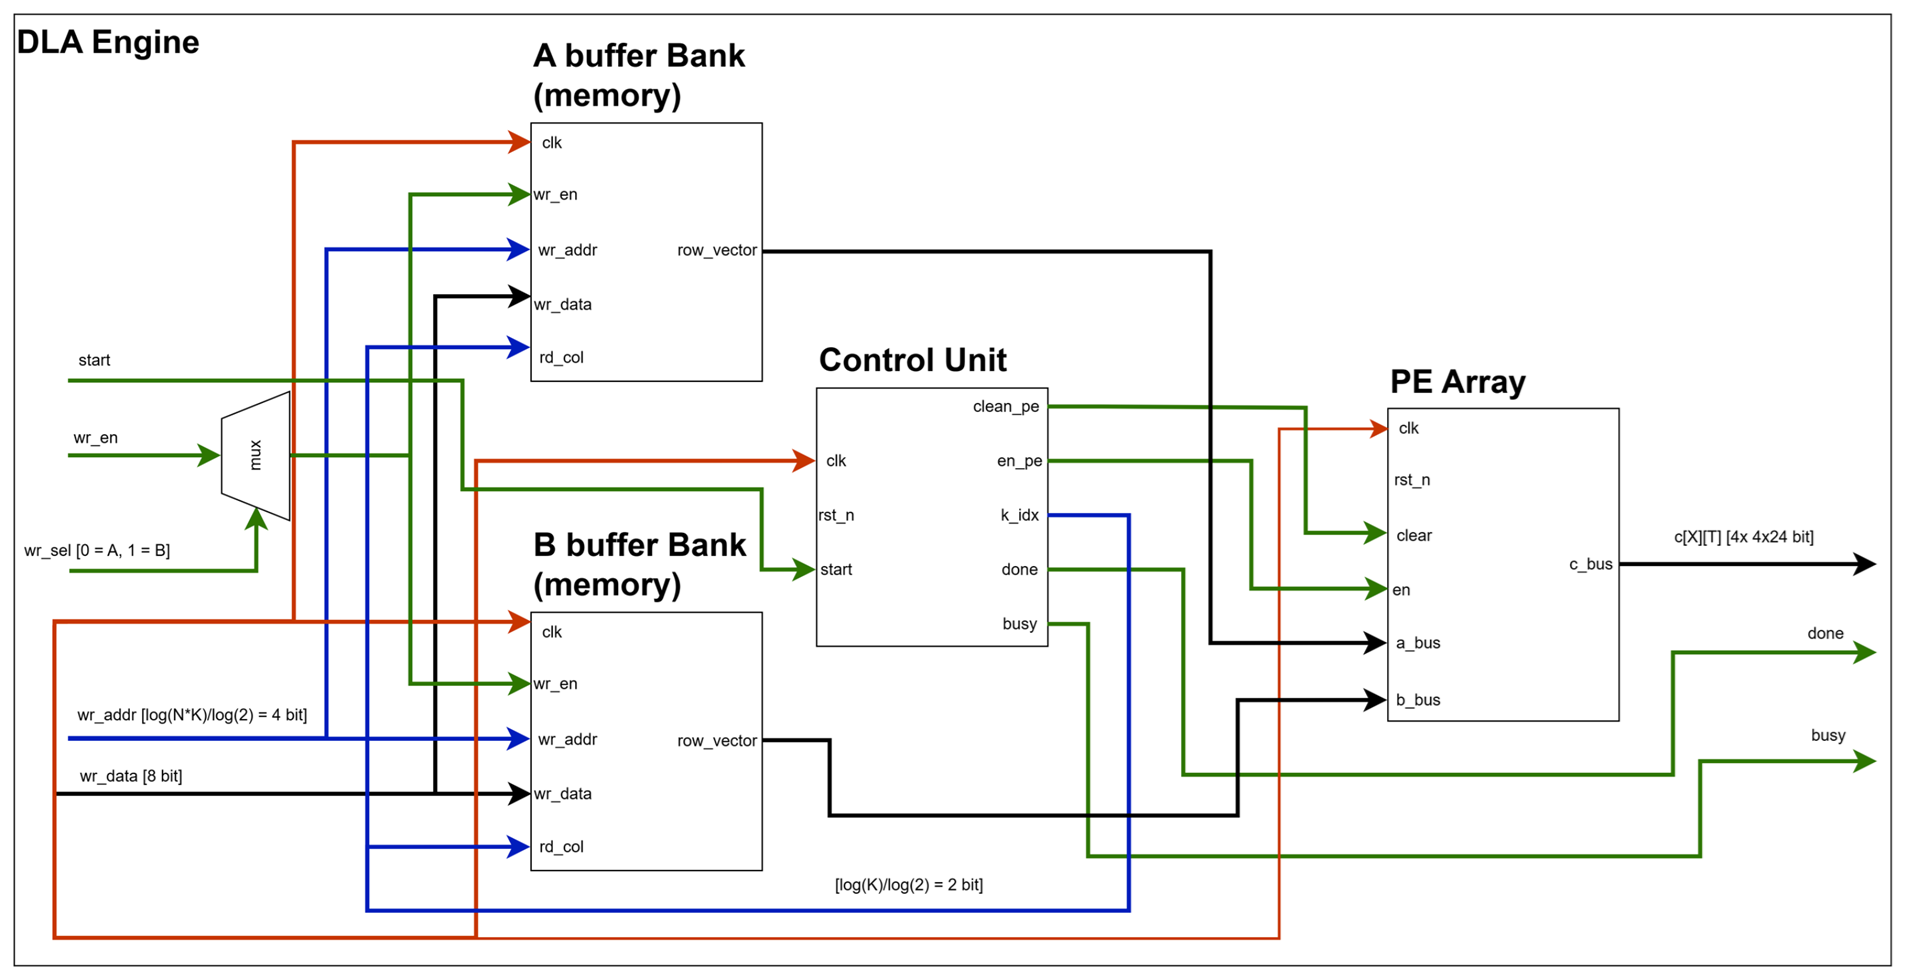
\includegraphics[width=0.98\columnwidth]{Top_level.png}
\caption{DLA engine top level.}
\label{fig:top}
\end{figure}

\subsection{PE Array and Controller}
Each PE (Fig.~\ref{fig:pe}, left) takes two signed 8-bit operands, multiplies them, sign-extends the 16-bit product to 24 bits, and adds it to a local accumulator,
\begin{equation}
acc[n]=acc[n-1]+a[n]\,b[n],
\end{equation}
so after $K$ cycles it holds one tile output; 24 bits give 256 accumulated 8-bit products enough range. The array (Fig.~\ref{fig:pe}, right) is 16 PEs in a $4\times4$ grid, each row fed one activation lane and each column one weight lane by broadcast, each PE accumulating locally --- output-stationary, all 16 in parallel, one tile per accumulation loop. The controller (Fig.~\ref{fig:fsm}) has four states: IDLE waits for START, CLEAR zeroes the accumulators, COMPUTE enables the array and increments the A and B addresses until all $K$ terms are consumed, DONE holds the completion flag until START falls. A writeback sequencer then serializes the accumulators into C and raises a writeback-done flag.

\begin{figure}[!ht]
\centering
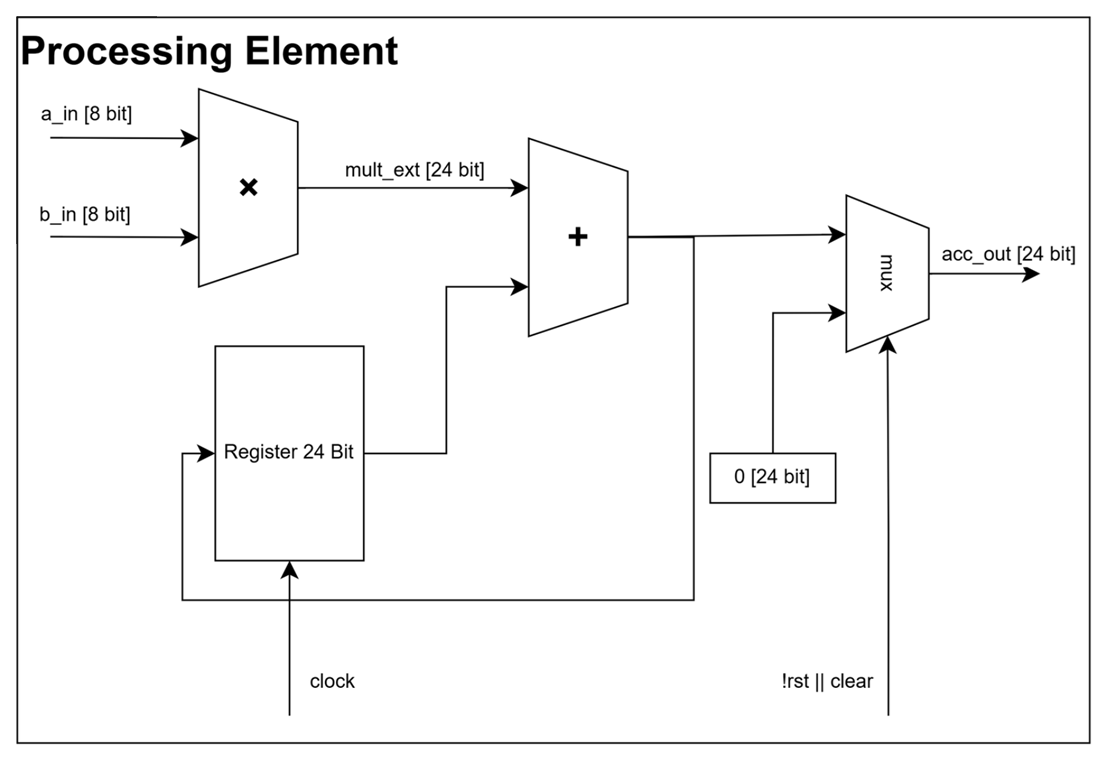
\includegraphics[width=0.46\columnwidth]{PE.png}\hfill
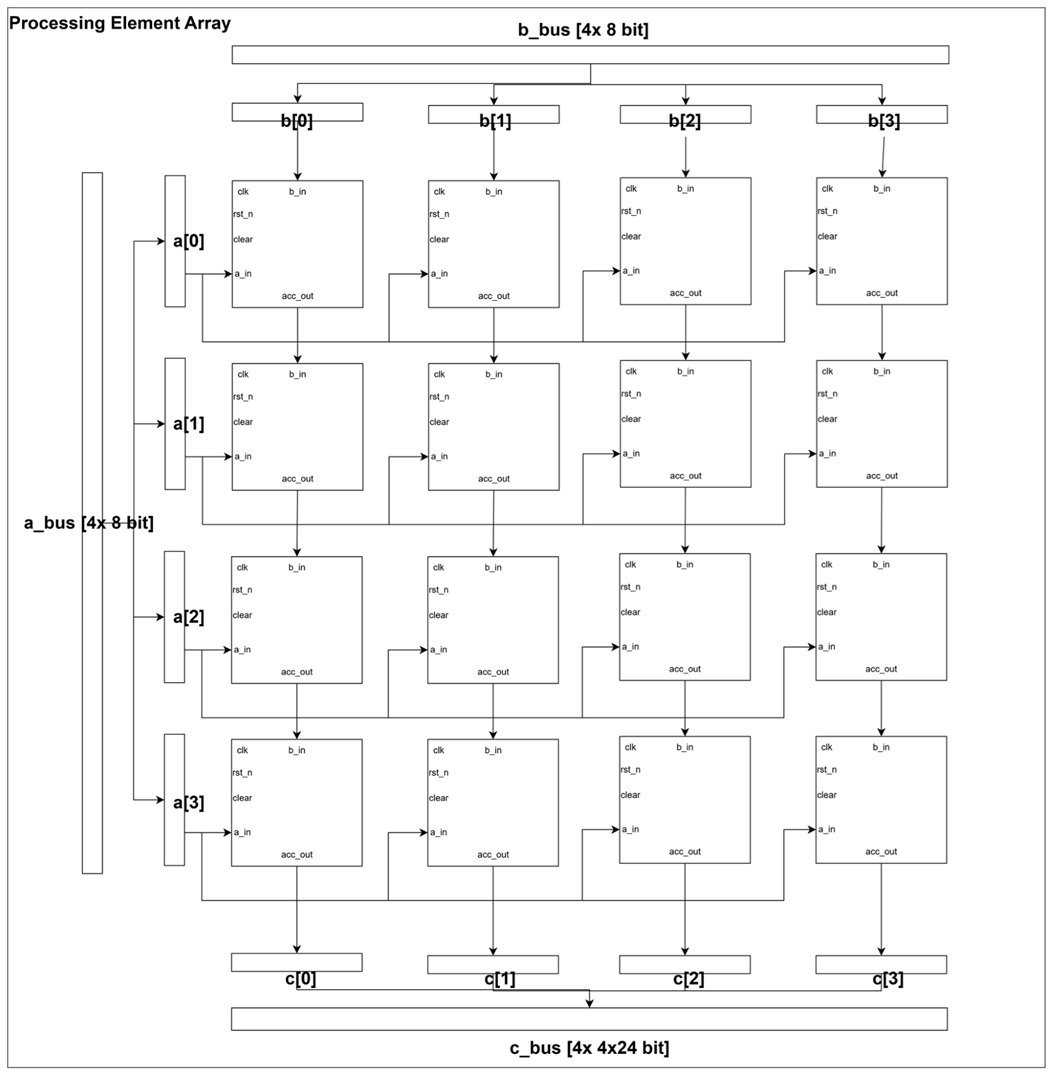
\includegraphics[width=0.50\columnwidth]{PE_Array.png}
\caption{Processing element datapath (left) and the $4\times4$ array (right).}
\label{fig:pe}
\end{figure}

\begin{figure}[!ht]
\centering
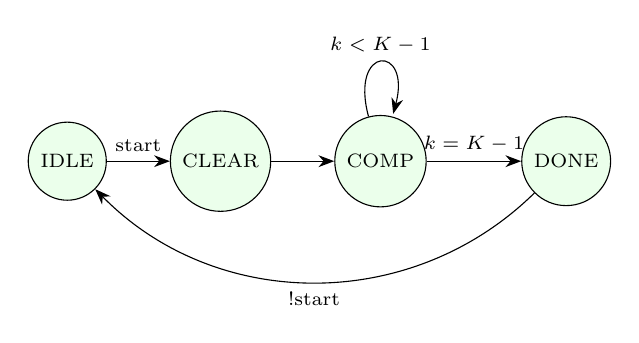
\begin{tikzpicture}[
  font=\scriptsize,>={Stealth[length=2mm]},
  st/.style={draw,circle,minimum size=9mm,fill=green!8}
]
\node[st] (idle) {IDLE};
\node[st,right=8mm of idle] (clear) {CLEAR};
\node[st,right=8mm of clear] (comp) {COMP};
\node[st,right=12mm of comp] (done) {DONE};
\draw[->] (idle) -- node[above]{start} (clear);
\draw[->] (clear) -- (comp);
\path (comp) edge[->,loop above] node{$k<K-1$} (comp);
\draw[->] (comp) -- node[above]{$k=K-1$} (done);
\draw[->] (done) to[bend left=45] node[below]{!start} (idle);
\end{tikzpicture}
\caption{Controller state machine.}
\label{fig:fsm}
\end{figure}

\subsection{SRAM Buffers}
The operand buffers are single-port SRAM macros: four $256\times8$ for A, one per row lane, and four for B, one per column. Eight is a bandwidth floor, not a capacity choice --- the array consumes four A and four B bytes per compute cycle from 1RW 8-bit parts, so no depth reduction reduces the count --- and both banks are exactly full at 1{,}024~bytes.

The C buffer is where the area was. It holds $N\times N=16$ accumulators of 24 bits --- 48 bytes --- which the predecessor stored as three $256\times8$ macros used as byte planes, bits [7:0], [15:8] and [23:16] sharing one address bus so a 24-bit word moved in one access. That spent 203{,}314~$\mu$m$^2$ on 48 bytes in 768, and no configuration of this array would ever use the rest: $C$ is $N\times N$ by construction.

This design folds the planes onto the address axis of one $64\times8$ macro, addressed as
\begin{equation}
\mathit{addr} = \mathit{word}\times 3 + \mathit{plane}, \quad \mathit{word}\in[0,16), \; \mathit{plane}\in[0,3),
\end{equation}
which uses 48 of 64 words and costs 45{,}861~$\mu$m$^2$ --- a 77\% reduction and two fewer macros to route around. Sixty-four is the shallowest depth this SRAM family offers, so this is the floor, not a tuning point. On-chip storage is nine macros and 2{,}112 bytes; the roughly 280~KB of INT8 weights stream through these tiles from outside.

The cost is that 24 bits no longer move in one access. The bank walks the planes itself: a write holds address and data steady and is acknowledged on the last plane, so writeback takes 48 cycles instead of 16 --- $+11.8\%$ against the 256 compute cycles it follows --- and a read assembles over three plane accesses plus the macro's registered latency, valid on the fourth cycle after the read enable rises. That latency is a contract every caller is written against (Section~\ref{sec:chip}). The wrapper carries a behavioral model for simulation and a blackbox branch for synthesis, power pins left to the PDN rather than tied in RTL; since the macro read has one cycle of latency, the top level delays the PE enable and completion flags by one cycle so the array never accumulates invalid data.

\section{Chip-Level Integration}\label{sec:chip}

The accelerator exposes 53 signal bits, but the shuttle slot gives only 20 general-purpose digital pads beside 60 analog, 8 supply, clock, and reset pads. Rather than a pin-per-signal map, the core wraps the accelerator behind a synchronous 4-wire serial bridge (SCLK, MOSI, CS\_N, MISO) that treats SCLK as data: all three inputs are double-flop synchronized and SCLK edge-detected, avoiding a second clock domain. Frames shift MSB-first while CS\_N is low --- 2-bit command, 10-bit address, plus 8 data bits on writes: WRITE\_A and WRITE\_B load the operand buffers, START launches a tile, READ\_C returns a 24-bit two's-complement result on MISO, and a rising CS\_N aborts safely. Three status flags (busy, done, writeback-done) drive pads directly for scope-visible liveness, so 9 of the slot's 91 pads are used. The folded C buffer is host-visible in one place only: a result assembles over three plane accesses, so the host leaves nine core clocks after the last address bit rather than four --- at SCLK~$\leq$~clk/8, one idle bit before the read data.

The padring is the wafer.space GF180MCU template \cite{padring} for a $2935\times2935~\mu$m workshop slot. It shorts the pad and core supplies into one rail on every pad, so the chip is single-supply by construction, and the operating point is 3.3~V for the whole die: logic and SRAM are 3.3~V parts and the foundry I/O cells are characterized at 3.3~V, so every cell runs in a foundry-characterized corner and the I/O levels suit a 3.3~V microcontroller host directly. The predecessor completed this flow with a clean chip-level sign-off, LVS over 71{,}668 instances included; \textbf{it has not yet been re-run against the nine-macro macro}, which is the next step and the reason this paper reports macro-level results.

\section{Software to Hardware Flow}\label{sec:sw}

The hardened core is the DLA engine alone; everything around it is a host (Fig.~\ref{fig:hwsoft}). In simulation that is Python plus a Verilog testbench preparing quantized weights, inputs, and reference outputs; on the finished chip, a microcontroller streaming the same tile schedule over the serial protocol.

\begin{figure}[!ht]
\centering
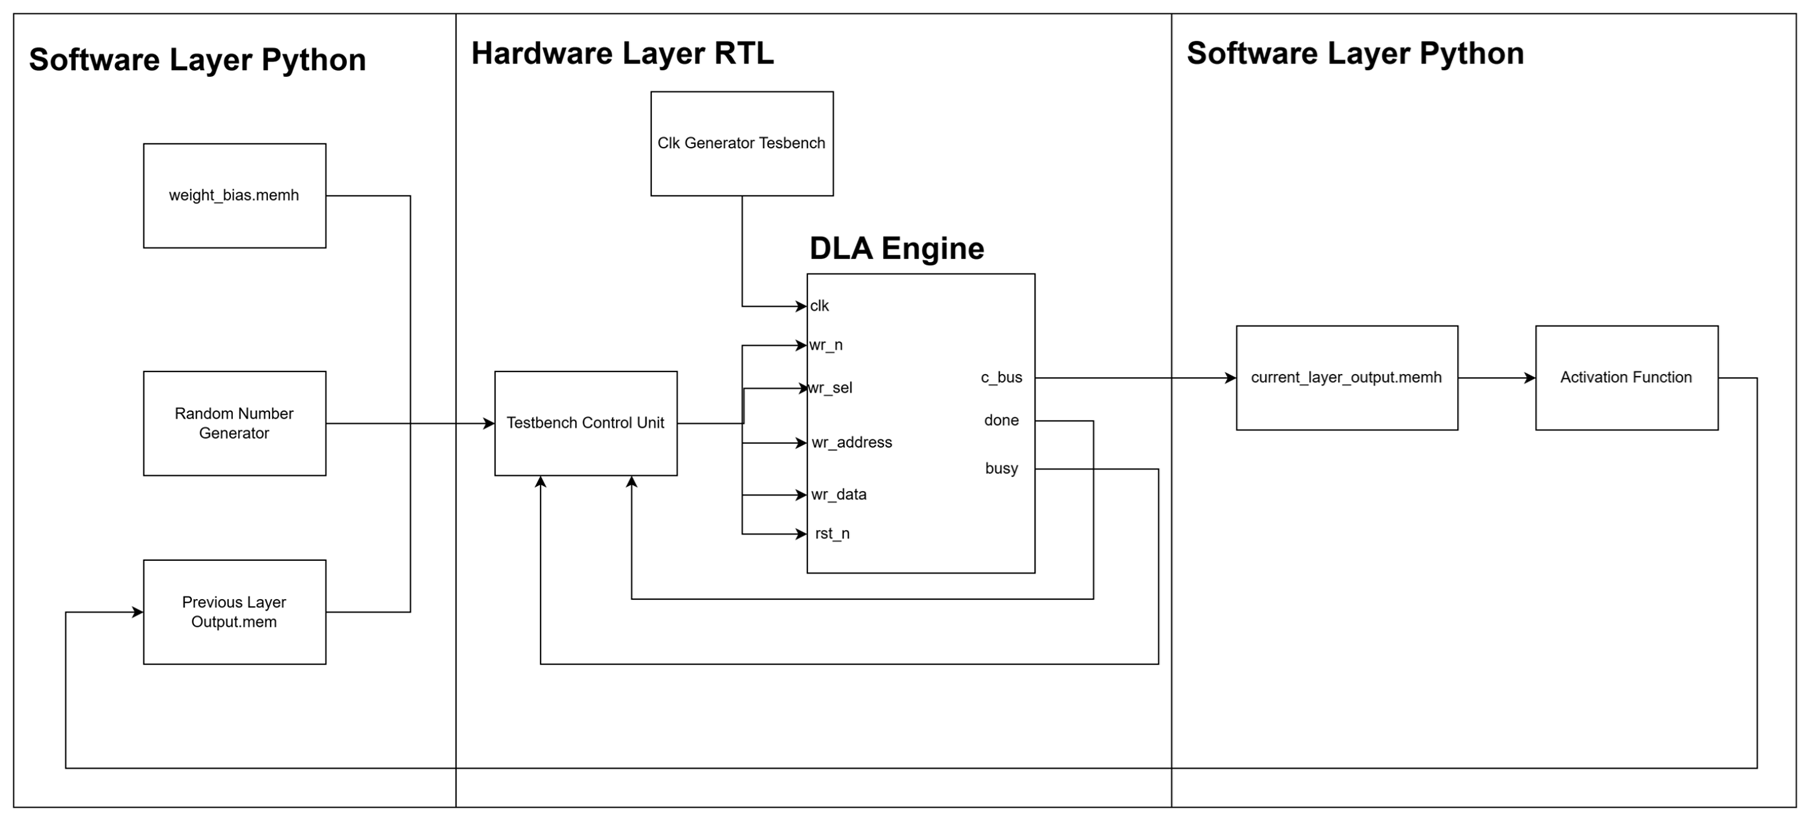
\includegraphics[width=0.94\columnwidth]{Hardware_Software_Integration.png}
\caption{Hardware and software flow.}
\label{fig:hwsoft}
\end{figure}

\subsection{Quantization and Requantization}
Every weight and bias tensor becomes signed 8-bit with one scale factor per tensor, taken from its largest absolute value and recorded in a manifest the testbench reuses. The DLA returns only a tile's integer dot product; the surrounding math is integer on the host, so hardware matches the Python reference exactly. Hidden-layer results are rescaled, biased, ReLU-activated, and requantized to 8 bits; output-layer results go to fixed point, through a tanh lookup table, to a grayscale pixel.

\subsection{Why INT8}\label{sec:format}

\begin{table}[!ht]
\caption{Numeric formats: accuracy against an exact FP64 render (10 latents, 7{,}840 pixels), and hardware cost. PE area is synthesized on the 3.3~V cells; accumulator width is what 256 accumulated products need.}
\label{tab:format}
\centering
\renewcommand{\arraystretch}{1.0}
\begin{tabular}{@{}lcccrc@{}}
\toprule
 & \multicolumn{2}{c}{Pixel error (gray levels)} & Weights & PE area & Acc. \\
\cmidrule(lr){2-3}
Format & mean & max & (KiB) & ($\mu$m$^2$) & (bits) \\
\midrule
INT4   & 22.26 & 255 & 138 & 6{,}245  & 15 \\
\textbf{INT8}  & \textbf{1.22} & \textbf{72} & \textbf{276} & \textbf{15{,}963} & \textbf{23} \\
INT16  & 0.01  & 1   & 552 & 47{,}037 & 39 \\
FP16   & 0.06  & 5   & 552 & ---      & --- \\
\bottomrule
\end{tabular}
\end{table}
Operand width sets multiplier area, buffer depth, and stream volume at once, so it was chosen by measurement: each format was applied to the same FP32 checkpoint and its render compared against an exact FP64 render of the same latent, against one PE's synthesized area at that width (Table~\ref{tab:format}). INT4 is not viable --- a per-tensor scale leaves seven magnitude steps, and 256 accumulated terms of that coarseness destroy the digit. INT16 is essentially exact but costs $2.95\times$ the PE area, a 39-bit accumulator, and double the weight traffic, which doubles time per image since streaming dominates latency (Section~\ref{sec:perf}). FP16 is no more accurate than INT16 for the same memory and a different datapath; none was built, so no area is quoted. INT8 sits at the knee: 1.2 gray levels of mean error is invisible in a $28\times28$ digit, the 16-bit product fits the 24-bit accumulator, and the width matches the SRAM word, so buffers need no packing logic.

\section{Verification}\label{sec:map}

The generator maps onto the DLA as tiled dense layers: per tile the four weight rows go to A and the shared input vector to B, the array performs the dot products, and the results land in C, one datapath serving every layer. Seven testbenches pass against Python golden vectors: one GEMM on a single lane; a full $N{=}4$/$K{=}256$ tile exercising every A and B macro; one layer row; a full 784-pixel image; the pad-level serial protocol driven as external hardware would; and gate-level re-simulations of the last two on the routed nine-macro netlist --- inserted buffers and roughly 8{,}100 antenna diodes included --- which reproduce the golden results bit-exactly, closing the gap between ``the RTL is correct'' and ``the taped-out netlist is correct.''

Folding the C buffer moved every testbench, and what broke was not obvious. The bank must restart its plane walk when the read \emph{address} changes, not only when the enable drops, or consecutive words interleave and a value assembles from two addresses. The serial bridge needs one wait cycle more than the on-chip caller, because it registers its read enable while the pipeline drives it combinationally, and must re-assert that pulse-type enable in the wait state. Testbenches need five clock edges where RTL callers need four. Each follows from turning one wide access into a sequence of narrow ones, and together they are the real cost of the fold --- larger than the 35 flip-flops it added.

The rendered digits (Fig.~\ref{fig:samples}) are limited in quality by the small generator and INT8 quantization, but confirm the full software-to-hardware path runs end to end.

\begin{figure}[!ht]
\centering

\includegraphics[width=0.15\linewidth]{digit_seed6.jpg}\hspace{3mm}

\includegraphics[width=0.15\linewidth]{digit_seed5.jpg}\hspace{3mm}
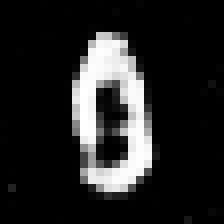
\includegraphics[width=0.15\linewidth]{digit_seed9.jpg}
\caption{Digits generated through the hardware path.}
\label{fig:samples}
\end{figure}

\section{Physical Implementation}\label{sec:phys}

The design is implemented with LibreLane \cite{librelane} on the GF180MCU open PDK \cite{gf180pdk}, hardened as a macro whose GDS/LEF/liberty views a padring integration consumes; everything below is that macro.

\subsection{Single-Supply 3.3~V Library Migration}
The buffer SRAM \cite{gf180sram} is a 3.3~V IP but the open PDK ships only 5~V cells, so a first version mixed a 5~V core with 3.3~V SRAMs --- fine for layout checks, level-shifted on silicon. Migrating to the third-party \texttt{gf180mcu\_as\_sc\_mcu7t3v3} native-3.3~V library, which ships nine liberty corners and a LibreLane integration, makes the die single-supply; bring-up surfaced three bugs in its flow integration (a missing timing-corner variable, a synthesis-exclusion filename mismatch, and non-synthesizable \texttt{\$random} initializers in six sequential-cell models that crashed lint), all fixed at the library source. The 3.3~V cells are far faster than the 5~V ones: the first run at 75~ns closed with $+44$~ns of setup slack, so the clock was retimed to 40~ns (25~MHz).

\subsection{Hardening the Accelerator Macro}

\begin{table}[!ht]
\caption{Antenna closure on the nine-macro die (40 ns, $1400\times1350~\mu$m). All runs are DRC-, LVS-, and timing-clean; only antenna varies. ``Structural'' marks a violator on a \texttt{GEN\_B\_COLS[1]} SRAM output.}
\label{tab:antenna}
\centering
\renewcommand{\arraystretch}{1.0}
\begin{tabular}{@{}llccl@{}}
\toprule
Placement & Density & Nets & Worst & Kind \\
\midrule
grid            & 63 & 1 & $2.18\times$ & structural \\
grid            & 59 & 2 & $1.73\times$ & marginal \\
grid            & 56 & 1 & $1.09\times$ & marginal \\
grid            & 54 & 1 & $1.10\times$ & marginal \\
grid            & 51 & 4 & $1.49\times$ & structural \\
\midrule
\textbf{B/C swap} & \textbf{56} & \textbf{0} & --- & \textbf{sign-off} \\
B/C swap        & 54 & 0 & --- & robustness \\
grid, margin 50 & 56 & 0 & --- & independent \\
\bottomrule
\end{tabular}
\end{table}
Four configuration points were essential: a synthesis define keeps the SRAM a hard macro (without it the memory is silently built from flip-flops); the macros are placed explicitly on a $3\times3$ grid with routing channels; the SRAM power pins reach only Metal3, so the macro power connection is made there; and routing runs to Metal5, with cell padding for diode access and diodes inserted at placement, in-router repair disabled.

Antenna closure is where the nine-macro floorplan behaved differently, and that difference is this paper's methodological result. In-router repair aborts in this flow --- its verification reroute fails pin access on already-placed clock-net diodes --- so closure must come from placement. On the eleven-macro design one density perturbation sufficed: it re-rolls which nets route long, and a single nudge cleared the lone marginal net.

Here it failed (Table~\ref{tab:antenna}): five densities across a twelve-point span, none reaching zero, settling into a basin at 54--56 with one net near $1.1\times$ and both directions worse. The sweep produced a diagnosis instead. The net names, which a count discards, all pointed one place: \texttt{GEN\_B\_COLS[1]}'s outputs were the $2.18\times$ structural violator at density 63 and returned at $1.49\times$ and $1.18\times$ at 51, while its eight neighbours never violated once. That macro sat in the grid corner furthest from the array, so its column broadcast crossed the whole die --- a placement error wearing an antenna costume. Swapping it into the centre and banishing the C buffer (48 bytes, a short net, never a violator) to the corner gave \textbf{zero violations} at no cost: $+16.46$ against $+16.11$~ns of setup slack, 145 fewer instances.

Two checks say fix, not lucky re-roll: the same swap is clean at density 54, where the unswapped floorplan sat at $1.10\times$, and holding the floorplan fixed while raising the pre-route diode margin from 25 to 50 reaches zero from the opposite direction --- two unrelated levers converging on those broadcast nets. The lesson: \emph{when a density sweep plateaus, stop sweeping and read the net names.} A violator surviving every density is not a lottery; the sweep's real output is its identity, not its count.

\begin{figure}[!ht]
\centering
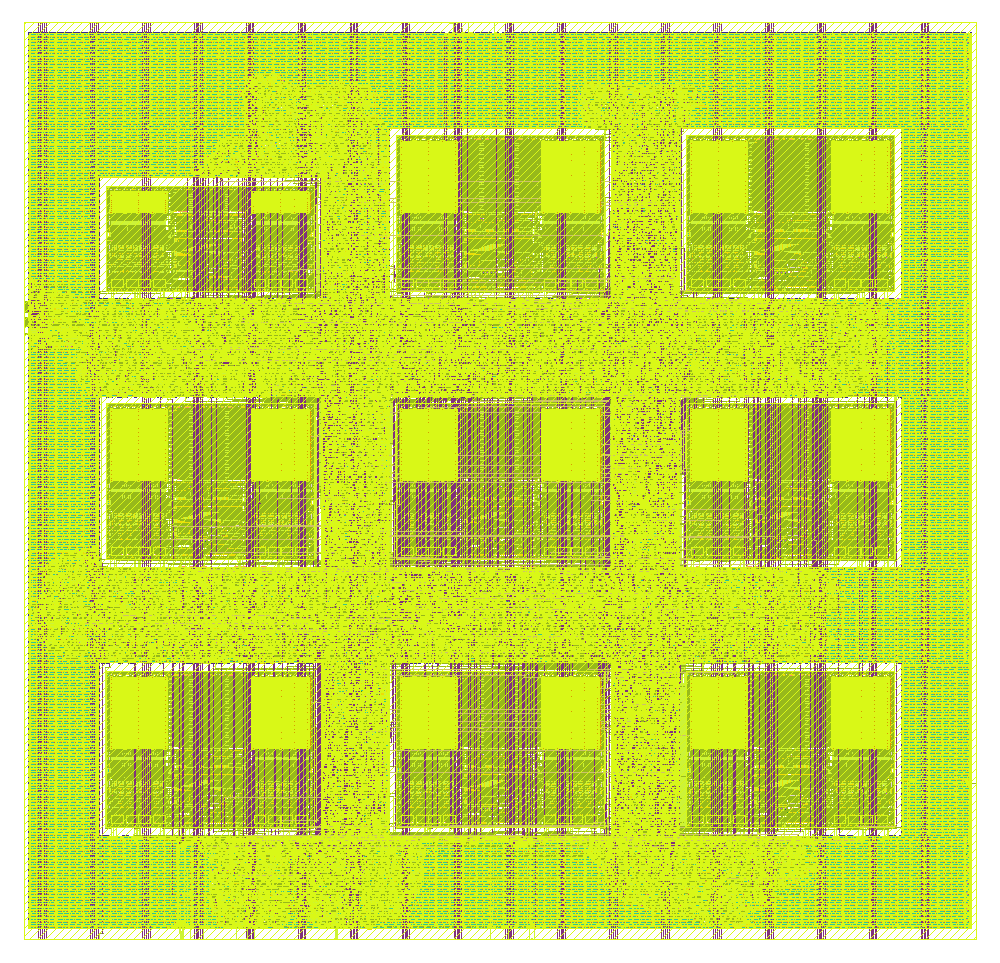
\includegraphics[width=0.52\columnwidth]{Tiny_GDS.png}
\caption{Hardened accelerator macro, $1375\times1325~\mu$m, with the nine SRAM macros on a $3\times3$ grid. The smaller block at the top left is the folded $64\times8$ C buffer, banished to the corner so that the antenna-violating B-buffer macro could take the centre slot.}
\label{fig:layout}
\end{figure}

With antenna closed, the die was squeezed. Runs at $1400\times1350$, $1375\times1325$ and $1350\times1300~\mu$m keep the swapped topology and scale only the die and macro coordinates, so channels tighten and nothing re-rolls. The middle size is promoted: 25~$\mu$m off each edge cost 0.22~ns of a 16~ns margin and \emph{saved} 2{,}171 instances --- looser placement carries more buffering, so tightening pays twice. The smallest is past the knee, two nets barely over at $1.04\times$ and $1.01\times$ and a density nudge worsening both directions ($1.75\times$ at 57, $1.31\times$ at 55): congestion, not a re-roll, so the squeeze stopped there.

Fig.~\ref{fig:layout} shows the resulting layout and Table~\ref{tab:vs11} the sign-off: zero Magic DRC errors, zero Netgen LVS errors, zero GDS XOR differences, zero violating antenna nets and pins, and the 40~ns clock met at all nine STA corners. The nominal 133~mW is almost entirely internal power estimated with the flow's default switching activity, and should be read as a conservative tool estimate rather than a measurement.

\subsection{Area and Timing Detail}\label{sec:areatiming}

\begin{table}[!ht]
\caption{Sign-off against the eleven-macro predecessor. Both are hardened on GF180MCU 180~nm at 3.3~V with the \texttt{gf180mcu\_as\_sc\_mcu7t3v3} cells at 40~ns, and both close with 0 DRC, 0 LVS, 0 XOR, and 0 antenna violations. Power is a tool estimate.}
\label{tab:vs11}
\centering
\renewcommand{\arraystretch}{1.0}
\begin{tabular}{@{}lrrr@{}}
\toprule
 & 11 macros & 9 macros & Change \\
\midrule
Die ($\mu$m)           & $1600{\times}1500$ & $1375{\times}1325$ & \\
Die area (mm$^2$)      & 2.400   & 1.822   & $-24\%$ \\
Core area (mm$^2$)     & 2.326   & 1.761   & $-24\%$ \\
SRAM area ($\mu$m$^2$) & 745,485 & 588,032 & $-21\%$ \\
C buffer ($\mu$m$^2$)  & 203,314 & 45,861  & $-77\%$ \\
Instances              & 93,172  & 79,676  & $-14\%$ \\
Power (mW)             & 162     & 133     & $-18\%$ \\
Wirelength (mm)        & 867     & 812     & $-6\%$ \\
Writeback (cycles)     & 16      & 48      & $+200\%$ \\
Compute per image (ms) & 3.54    & 3.95    & $+11.7\%$ \\
Setup slack, worst (ns) & $+15.12$ & $+16.24$ & better \\
Hold slack, worst (ns)  & $+0.150$ & $+0.116$ & thinner \\
Clock skew, worst (ns)  & 0.65    & 0.44    & $-32\%$ \\
Critical path (ns)      & 24.88   & 23.76   & $-4\%$ \\
\bottomrule
\end{tabular}
\end{table}

The core area shows what the fold achieved and what it did not. Nine macros take 0.588~mm$^2$ against 0.745~mm$^2$: a 21\% cut of SRAM area from a 77\% cut of one buffer. The floorplan stays memory-dominated --- macros 33.4\% of the core against 21\% for all placed cells --- since the eight A and B macros are a bandwidth floor and cannot be folded. Arithmetic is a minority of the logic: 0.242~mm$^2$ combinational against 0.038~mm$^2$ of well taps, 0.036~mm$^2$ of 8{,}145 diodes, and 39.0\% fill and decap. Sequential area rises from 406 to 441 flip-flops, the plane-walking state machine --- 35 flip-flops bought 157{,}453~$\mu$m$^2$ of macro.

Timing signs off at nine corners --- three PVT points crossed with minimum, nominal, and maximum interconnect --- with zero violations, setup set by the slow corner (SS, 125\,\textdegree C, 3.0~V; $+16.24$~ns) and hold by the fast one (FF, $-40$\,\textdegree C, 3.6~V; $+0.116$~ns). The area reduction \emph{improved} setup, $+16.24$ against $+15.12$~ns, because a smaller die shortens the nets the critical path runs on: SRAM read, operand multiplexing, MAC, accumulator register --- putting A and B in SRAM is what places a macro read on a combinational path, and at the slow corner its clock-to-output is 12.6--15.0~ns of the total. The remaining slack puts the true critical path at 23.76~ns, closing near 42~MHz; 25~MHz is a deliberate $1.7\times$ guard band on a first tapeout in an unfamiliar library. Hold, the thinnest number in the sign-off, is set by clock-tree skew (0.44~ns), not the period.

Table~\ref{tab:vs11} collects the comparison: the fold pays on every physical axis at once --- 24\% of the die, 21\% of the SRAM area, 14\% of the instances, 18\% of the power --- and improves setup margin rather than trading against it. It costs cycles in one place only: writeback grows from 16 to 48 cycles per transaction, 11.7\% more compute per image and 0.04\% of end-to-end latency (Section~\ref{sec:perf}).

\section{Performance}\label{sec:perf}

\subsection{Latency Breakdown}

\begin{table}[!ht]
\caption{End-to-end latency for one $28\times28$ image at a 25~MHz core clock and SCLK of 3.125~MHz (clk/8). On-chip cycles are measured from the full-image simulation; link times follow from the protocol's frame lengths at that rate.}
\label{tab:latency}
\centering
\renewcommand{\arraystretch}{1.0}
\begin{tabular}{@{}lrrr@{}}
\toprule
Stage & Frames & Time (ms) & Share \\
\midrule
Weight tiles $\rightarrow$ A buffer & 331{,}776 & 2{,}123.4 & 98.85\% \\
Input vector $\rightarrow$ B buffer & 768       & 4.9       & 0.23\% \\
START commands                      & 324       & 1.2       & 0.06\% \\
Compute + writeback (on chip)       & 324 tiles & 4.0       & 0.18\% \\
Result readback from C              & 1{,}296   & 15.3      & 0.71\% \\
\midrule
Total                               &           & 2{,}149   & 0.47 img/s \\
\bottomrule
\end{tabular}
\end{table}
The array performs 16 MAC operations per cycle, a peak of 0.8~GOPS at 25~MHz; quoting only that would be misleading, so this section separates what the array costs from what feeding it costs. On-chip cycle counts are instrumented per controller state in the full-image simulation; link times follow from the frame lengths of Section~\ref{sec:chip}.

Per tile the engine is busy 305 cycles: one CLEAR, 256 accumulation, and 48 writeback cycles walking sixteen accumulators through three byte planes. Over 324 tiles that is 98{,}820 cycles, 3.95~ms at 40~ns --- pure compute, 17.9\% of peak, against 3.54~ms and 20.0\% for the eleven-macro design; the 11.7\% penalty is exactly the writeback growth. The shortfall from peak is structural: the generator evaluates a matrix--\emph{vector} product, so only the four PEs of B's first column produce useful neurons while twelve recompute against unused columns, and batching four latents recovers most of it with no hardware change. Feeding the array costs far more: each tile needs four weight rows across the full $K=256$ depth, 1{,}024 bytes, each byte one 20-bit frame at SCLK~$\leq$~clk/8 --- 3.125~MHz, 6.4~$\mu$s per byte (Table~\ref{tab:latency}).

End-to-end latency is therefore \textbf{2.149~s per image} (0.47 images/s) against 4.0~ms of arithmetic: the link is 99.8\% of it, weight streaming alone 98.8\%, an effective 263~kOPS. This settles the area trade --- the folded buffer costs 0.41~ms of compute and 0.41~ms of slower reads, together 0.04\% of an image, and buys 24\% of the die. The bottleneck is not link width but zero weight reuse: a matrix--vector product touches every weight once, so 1.01 bytes cross per MAC however the interface is built, and even an idealized parallel port at one byte per core clock leaves weight loading at 331{,}776 of 440{,}903 cycles, 75\%. Some traffic is avoidable: the schedule writes the full 256-deep A tile even for L0, whose inputs are 64 wide, so a host pre-zeroing the tail sends 282{,}624 bytes and finishes in 1.83~s. This is the trade the pad budget forced --- 20 pads and 2.1~KB of SRAM against 280~KB of weights --- and where future work belongs: a burst write sending the address once removes 12 of every 20 bits.

\subsection{Comparison}

\begin{table}[!ht]
\caption{Comparison with representative accelerators. Throughput is peak ($2\times$ MACs $\times$ frequency); efficiency is peak throughput over reported power. Our power is a tool estimate.}
\label{tab:compare}
\centering
\small
\renewcommand{\arraystretch}{1.12}
\begin{tabular}{@{}lccrrc@{}}
\toprule
 & Tech. & Area & Peak & Eff. & Open \\
Design & (nm) & (mm$^2$) & (GOPS) & (GOPS/W) & flow \\
\midrule
DianNao \cite{diannao}   & 65  & 3.02  & 452   & 932 & No \\
Eyeriss \cite{eyeriss}   & 65  & 12.25 & 67.2  & 242 & No \\
Wang \emph{et al.} \cite{wang} & 40 & 11.97 & 54.61 & 567 & No \\
OpenSpike \cite{openspike} & 130 & 33.3 & ---   & 56.8 & Yes \\
\textbf{This work}       & 180 & \textbf{1.76} & 0.8 & 6.0 & \textbf{Yes} \\
\bottomrule
\end{tabular}
\end{table}
Table~\ref{tab:compare} places this work against three fabricated commercial-node accelerators \cite{diannao, eyeriss, wang} and one open-PDK, open-flow tapeout \cite{openspike}, on peak figures so different scales compare on one basis. The gap reads plainly: two to three orders of magnitude below the commercial parts in throughput, about two in efficiency, almost none of it architectural. A $4\times4$ array at 25~MHz has $31\times$ fewer multipliers than Eyeriss at $8\times$ the clock, which alone accounts for throughput; the efficiency gap is what 180~nm at 3.3~V costs. The isolating comparison is OpenSpike: at similar scale and clock this design occupies 1.76~mm$^2$ against 33.3~mm$^2$, on foundry hard SRAM macros rather than generated memory. What this work offers is reproducibility and density, not performance.

\section{Conclusion}\label{sec:concl}
This work makes a signed-off INT8 GAN-generator accelerator on GF180MCU 24\% smaller by questioning its memory rather than its logic. Folding the result buffer's three byte planes onto the address axis of one $64\times8$ macro cuts that buffer 77\%, removes two macros, and allows a $3\times3$ arrangement on a $1375\times1325~\mu$m die drawing 18\% less power and closing with \emph{more} setup margin, for 11.7\% more compute cycles, 0.04\% of end-to-end latency. Both results generalize. Buffer depth and \emph{shape} are separable: byte planes spend one macro per byte of word width, the floorplan pays for macro count rather than occupancy, and folding planes onto the address axis trades width for latency --- attractive for any accumulator buffer off the critical path whose depth is fixed by array geometry. And a density sweep is a re-roll, not an optimization: five densities gave no zero but one consistent net name, and acting on it closed antenna in one run. The macro passes DRC, LVS, XOR, and antenna cleanly at 40~ns across nine corners on one 3.3~V supply, verified bit-exactly to a full-image render on the routed netlist. The limits are unchanged: a tile engine with no weight reuse is interface-bound at any width, so batching latents through the unused columns, a burst write, and a wider bus are the levers, none a datapath change. Next is the padring integration, then silicon.

\section*{Acknowledgment}
The authors thank the open-source EDA community, the GlobalFoundries open PDK program, and the wafer.space chipathon program.

\begin{thebibliography}{15}
\setlength{\itemsep}{0pt}
\bibitem{tpu} N. P. Jouppi \emph{et al.}, ``In-datacenter performance analysis of a tensor processing unit,'' in \emph{Proc. ISCA}, 2017.
\bibitem{survey} C. Silvano \emph{et al.}, ``A survey on deep learning hardware accelerators for heterogeneous HPC platforms,'' \emph{ACM Computing Surveys}, 2025.
\bibitem{diannao} T. Chen \emph{et al.}, ``DianNao: a small-footprint high-throughput accelerator for ubiquitous machine learning,'' \emph{Proc. ASPLOS}, 2014.
\bibitem{eyeriss} Y.-H. Chen, T. Krishna, J. S. Emer, and V. Sze, ``Eyeriss: an energy-efficient accelerator for deep convolutional neural networks,'' \emph{IEEE JSSC}, vol.~52, no.~1, pp.~127--138, 2017.
\bibitem{openspike} F. Modaresi, M. Guthaus, and J. K. Eshraghian, ``OpenSpike: an OpenRAM SNN accelerator,'' in \emph{Proc. IEEE ISCAS}, 2023.
\bibitem{jacob} B. Jacob \emph{et al.}, ``Quantization and training of neural networks for integer-arithmetic-only inference,'' \emph{Proc. CVPR}, 2018.
\bibitem{wang} C. C. Wang \emph{et al.}, ``A 54.61 GOPS 96.35 mW digital logic accelerator for underwater object recognition DNN in 40 nm CMOS,'' in \emph{Proc. IEEE AICAS}, 2024.
\bibitem{goodfellow} I. Goodfellow \emph{et al.}, ``Generative adversarial nets,'' in \emph{Proc. NeurIPS}, 2014.
\bibitem{ganpretrained} C. Singh, ``GAN/VAE pretrained PyTorch models,'' \url{github.com/csinva/gan-vae-pretrained-pytorch}.
\bibitem{dlaengine} ``DLA Engine,'' GitHub, \url{github.com/wlmoi/DLA_Engine}.
\bibitem{padring} wafer.space, ``GF180MCU project template,'' \url{github.com/wafer-space/gf180mcu-project-template}.
\bibitem{librelane} ``LibreLane: an open-source RTL-to-GDSII flow,'' \url{github.com/librelane/librelane}.
\bibitem{gf180pdk} GlobalFoundries and Google, ``GF180MCU open-source PDK,'' \url{github.com/google/gf180mcu-pdk}.
\bibitem{gf180sram} R. T. Edwards, ``GF180MCU OCD IP SRAM macros,'' \url{github.com/RTimothyEdwards/gf180mcu_ocd_ip_sram}.
\end{thebibliography}

\end{document}